\documentclass{sigchi-ext}
% Please be sure that you have the dependencies (i.e., additional
% LaTeX packages) to compile this example.
\usepackage[T1]{fontenc}
\usepackage{textcomp}
\usepackage[scaled=.92]{helvet} % for proper fonts
\usepackage{graphicx} % for EPS use the graphics package instead
\usepackage{balance}  % for useful for balancing the last columns
\usepackage{booktabs} % for pretty table rules
\usepackage{ccicons}  % for Creative Commons citation icons
\usepackage{ragged2e} % for tighter hyphenation

% Some optional stuff you might like/need.
% \usepackage{marginnote} 
% \usepackage[shortlabels]{enumitem}
% \usepackage{paralist}
% \usepackage[utf8]{inputenc} % for a UTF8 editor only

%% EXAMPLE BEGIN -- HOW TO OVERRIDE THE DEFAULT COPYRIGHT STRIP --
% \copyrightinfo{Permission to make digital or hard copies of all or
% part of this work for personal or classroom use is granted without
% fee provided that copies are not made or distributed for profit or
% commercial advantage and that copies bear this notice and the full
% citation on the first page. Copyrights for components of this work
% owned by others than ACM must be honored. Abstracting with credit is
% permitted. To copy otherwise, or republish, to post on servers or to
% redistribute to lists, requires prior specific permission and/or a
% fee. Request permissions from permissions@acm.org.\\
% {\emph{CHI'14}}, April 26--May 1, 2014, Toronto, Canada. \\
% Copyright \copyright~2014 ACM ISBN/14/04...\$15.00. \\
% DOI string from ACM form confirmation}
%% EXAMPLE END

% Paper metadata (use plain text, for PDF inclusion and later
% re-using, if desired).  Use \emtpyauthor when submitting for review
% so you remain anonymous.
\def\plaintitle{Examining Marginalization in the Financial Industry Related to Conversational Agents}
\def\plainauthor{Christina Wei, Anastasia Kuzminykh}
\def\emptyauthor{}
\def\plainkeywords{conversational user interfaces; chatbot; financial industry;  marginalization}
\def\plaingeneralterms{conversational user interfaces; chatbot; financial industry;  marginalization}

\title{Examining Marginalization in the Financial Industry Related to Conversational Agents}

\numberofauthors{2}
% Notice how author names are alternately typesetted to appear ordered
% in 2-column format; i.e., the first 4 autors on the first column and
% the other 4 auhors on the second column. Actually, it's up to you to
% strictly adhere to this author notation.
\author{%
  \alignauthor{%
    \textbf{Christina Wei}\\
    \affaddr{University of Toronto} \\
    \affaddr{Toronto, Canada} \\
    \email{christina.wei@mail.utoronto.ca}
  } 
  \vfil
  \alignauthor{%
    \textbf{Anastasia Kuzminykh}\\
    \affaddr{University of Toronto}}\\
    \affaddr{Toronto, Canada} \\
    \email{anastasia.kuzminykh@utoronto.ca}
}

% Make sure hyperref comes last of your loaded packages, to give it a
% fighting chance of not being over-written, since its job is to
% redefine many LaTeX commands.
\definecolor{linkColor}{RGB}{6,125,233}
\hypersetup{%
  pdftitle={\plaintitle},
%  pdfauthor={\plainauthor},
  pdfauthor={\emptyauthor},
  pdfkeywords={\plainkeywords},
  bookmarksnumbered,
  pdfstartview={FitH},
  colorlinks,
  citecolor=black,
  filecolor=black,
  linkcolor=black,
  urlcolor=linkColor,
  breaklinks=true,
}

% \reversemarginpar%

\begin{document}

%% For the camera ready, use the commands provided by the ACM in the Permission Release Form.
\CopyrightYear{2022}
\setcopyright{rightsretained}
\conferenceinfo{CHI'23,}{April  23--28, 2023, Hamburg, Germany}
\isbn{978-1-4503-6819-3/20/04}
\doi{https://doi.org/10.1145/3334480.XXXXXXX}
%% Then override the default copyright message with the \acmcopyright command.
\copyrightinfo{\acmcopyright}


\maketitle

% Uncomment to disable hyphenation (not recommended)
% https://twitter.com/anjirokhan/status/546046683331973120
\RaggedRight{} 

% Do not change the page size or page settings.
\begin{abstract}
Currently, the deployment of conversational agents in the financial sector is predominately focused on handling transactional inquiries in the customer service domain. This approach is associated with the issues of marginalizing customer service employees by reinforcing the societal bias of ``low-value'' work, dehumanizing and concealing their labour behind machines, and reinforcing gender and professional stereotypes. Furthermore, the deployment of these conversational agents contributes to product differentiation based on wealth by digitizing services for general customers. In light of these problems, we advocate for leveraging conversational agents' capabilities for more inclusive design and discuss the corresponding avenues.
\end{abstract}

\keywords{\plainkeywords}

% ACM Classfication

\begin{CCSXML}
<ccs2012>
<concept>
  <concept_id>10003120.10003121</concept_id>
  <concept_desc>Human-centered computing~Human computer interaction (HCI)</concept_desc>
  <concept_significance>500</concept_significance>
</concept>
<concept>
    <concept_id>10003120.10003121.10003124.10010870</concept_id>
    <concept_desc>Human-centered computing~Natural language interfaces</concept_desc>
    <concept_significance>500</concept_significance>
</concept>
</ccs2012>
\end{CCSXML}

\ccsdesc[500]{Human-centered computing~Human computer interaction (HCI)}
\ccsdesc[500]{Human-centered computing~Natural language interfaces}

% Print the classficiation codes
\printccsdesc
%Please use the 2012 Classifiers and see this link to embed them in the text: %\url{https://dl.acm.org/ccs/ccs_flat.cfm}


\section{Introduction}

Financial decisions are among the most complex and consequential decisions we make in our lives. Many individuals need assistance to make these decisions, e.g. the majority of Americans are feeling anxious about their financial situation \cite{capitalone2020}. The advancements in financial technology (FinTech), such as the introduction of robo-advisors\footnote{https://www.investopedia.com/terms/r/roboadvisor-roboadviser.asp} helps to commoditize personal advice services that were previously only accessible to high-net-worth customers \cite{philippon2019fintech}. Conversational agents also have the potential to improve financial inclusion, as their ability to communicate with users using natural language is well suited to support users in their decision-making process \cite{volkel2021eliciting}. However, the opportunities to create chatbots for more complex decision-making tasks like financial decisions are still largely under-explored \cite{reicherts2022extending}. Instead, financial industry has mainly focused on deploying chatbots to handle transactional inquiries in the customer service context, such as Eno the Capital One Assistant\footnote{https://www.capitalone.com/digital/eno/}. While these agents are beneficial for financial institutions, they lead to discrimination problems within the industry as well as for customers.

In this paper, we first spotlight the issue of conversational agents marginalizing customer service employees through the augmentation of their work. We then discuss the role of these agents in reinforcing the existing structure of wealth-based service differentiation
%, widening the access gap to personalized support 
between general and high-net-worth customers. Lastly, we highlight areas where conversational agents can be employed to increase financial inclusion.


\section{Marginalization of Human Labour}

\begin{marginfigure}[-17pc]
  \begin{minipage}{\marginparwidth}
    \centering
    
\includegraphics[width=0.8\marginparwidth]{figures/chatbot.png}
    \caption{Banking and finance conversational agents from Chatbot Guide \cite{chatbotguide}}
    \label{fig:chatbots}
  \end{minipage}
\end{marginfigure}

Surveying the landscape conversational agents used in banking and finance, most companies are implementing chatbots to support transactional inquiries such as checking account balances or making payments \cite{chatbotguide}. The collective decision made by financial institutions to augment transactional customer service capabilities with virtual agents is the reification of labour politics that is pervasive in our culture. Our social prejudice perceives customer service as low-value and repetitive work that can be automated more easily than the higher value work done by financial advisors \cite{dhaliwal2022cyber}. Because of their lower social status, customer service workers have limited ability to fight back against the augmentation of their jobs. However, if one objectively analyzes the tasks performed by financial advisors and customer service workers, both roles have elements that can be automated by machines. The augmentation of customer services with conversational agents also creates a dangerous self-reinforcing cycle. Because customer service is perceived as low-value work, more automations are deployed to augment their capabilities. With more automated capabilities, they perpetuate the stereotype that customer service labour is of low value and can be augmented by machines. Additionally, automations introduce the issue of hiding human labour behind conversational agents.

There are ethical concerns with the representation of customer service labour through conversational agents. Grudin and Jacques \cite{grudin2019chatbots} discussed the issues in human-chatbot teams for human agents to jump in and handle inquiries that conversational agents are unable to answer. If conversational agents are not designed properly, customers may not be able to distinguish between human vs. virtual agents, therefore mistakenly attributing human labour to machines. In some cases, companies may be deliberately hiding human labour behind the facade of conversational agents, disguising customer service representatives' work as the algorithms of the agents. Also, there is the problem with conversational agents' portrayals of customer service representatives. Based on the 34 chatbots listed in Chatbot Guide for Banking and Finance Industry \cite{chatbotguide} (\autoref{fig:chatbots}), most of the agents are represented using abstract avatars or company logos. The lack of human resemblance in these chatbots dehumanizes the role of customer service representatives, treating them as commodities that are indistinguishable and interchangeable with one another. Out of the conversational agents listed in Chatbot Guide \cite{chatbotguide}, five of them used typical female names (Erica from Bank of America\footnote{https://www.chatbotguide.org/bank-of-america-bot}, Sara from Commercial Bank of Dubai\footnote{https://www.chatbotguide.org/commercial-bank-of-dubai-bot}, Ada from Diamond Bank\footnote{https://www.chatbotguide.org/diamond-bank-bot}, Eva from HDFC Bank\footnote{https://www.chatbotguide.org/hdfc-bot}, and Hannah from M\&S Bank\footnote{https://www.chatbotguide.org/ms-bank-bot}) compared to only one agent using a typical male name (Lionel from ING\footnote{https://www.chatbotguide.org/ing-bot}). Some agents using female names are also linked to human-like avatars that are depicted using conventionally female traits (\autoref{fig:female-avatars}). This analysis illustrates the prejudice inherent in the selection of female personas for conversational agents, which may be perpetuating harmful gender stereotypes such as attributing subservient attitudes to customer service employees \cite{ruane2019conversational}.

\begin{marginfigure}[3pc]
  \begin{minipage}{\marginparwidth}
    \centering
    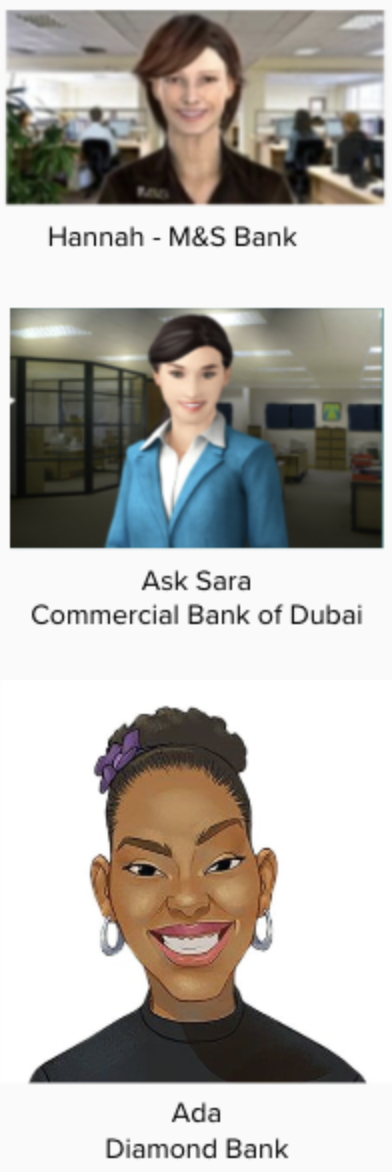
\includegraphics[width=0.8\marginparwidth]{figures/avatars.png}
    \caption{Banking and finance bots using female avatars}
    \label{fig:female-avatars}
  \end{minipage}
\end{marginfigure}


\section{Reinforcing Wealth-Based Service Differentiation}

The segregation of financial services between general customers and high-net-worth individuals is reinforced by conversational agents. %augmenting customer service capabilities. 
Typically, virtual agents are developed for services offered to general customers, producing profitable returns on investment for frequently asked questions. Dedicated services provided to high-net-worth individuals are usually not augmented by conversational agents, as their value proposition is to build personal relationships with customers through white-glove services. The notion that these specialized and dedicated services can be automated by virtual assistants diminishes their perceived value. As such, there is a divide between the digitization of the services available to general customers and the personalized services offered to high-net-worth individuals. For general customers, it is common to be interfacing with automated algorithms as the first interaction point. For example, when calling into contact centers, customers need to first navigate through an Interactive Voice Response (IVR) system before they can reach a human customer service representative. Similarly, conversational agents are being advertised and used as the first point of contact to help customers on digital channels \cite{revechat}. A customer will only be transferred to a human representative if the virtual agent's algorithm determines that it cannot handle the client's inquiry. This reduces the access to personalized help for general customers, potentially limiting flexibility on their financial products. These limitations do not apply for high-net-worth individuals as they have access to dedicated teams to assist them with their financial needs. Thus, digital tools like conversational agents are reinforcing and potentially deepening the divide in services between general and high-net-worth customers.


\section{Moving Towards Inclusive Design}

While the current implementations of conversational agents have marginalizing effects in the financial industry, they can also be used for more inclusive design. One potential use case is to utilize virtual agents to lessen the access segregation of financial products. In financial services, many products are transacted through intermediaries, such as financial advisors purchasing mutual funds on behalf of their customers. Customers' access to financial products depend on intermediaries' regulatory licenses and product coverage. For example, a broker may be licensed to offer insurance products and not mutual funds, but their clients may not be aware of this limitation and potentially missing access to a broader range of products. Conversational agents can be used to educate customers on the full spectrum of financial products that are available in the market, as well as connect them with appropriate financial intermediaries to address their financial needs. Also, as conversational agents evolve to handle more complicated conversations, we can implement more personalized advice solutions for general customers that are historically only available to high-net-worth individuals, thus reducing the gap of wealth-based service differentiation. This work is already happening in FinTech through robo-advisor capabilities \cite{philippon2019fintech}. We can further assist users with their financial decision-making by augmenting these services using conversational agents. 


\section{Closing Remarks}

This paper discusses various aspects of marginalization by conversational agents in the financial industry. Specifically, there are marginalizing effects for both users of conversational agents and the workers whose jobs are affected by these agents. We can leverage Sin et al.\cite{sin2021digital}'s digital design marginalization framework to avoid digitally marginalizing groups of users and to design inclusive digital interfaces. We implore the conversational user interface community to investigate agents that help users make financial decisions to bridge the wealth-based access gap, as well as agents that empower customer service representatives in their profession and safeguard them from social prejudices.
%To close the wealth-based access gap for individualized financial advice, we urge the conversational user interface community to explore agents that assist users in their financial decision-making process.
%Specifically for the financial industry, we urge the conversational user interface community to investigate agents supporting users in their financial decision-making process in order to narrow the wealth-based access gap for personalized financial advice.

\balance{} 

\bibliographystyle{SIGCHI-Reference-Format}
\bibliography{reference}

\end{document}

%%% Local Variables:
%%% mode: latex
%%% TeX-master: t
%%% End:
